\documentclass[stu,hidelinks,floatsintext,donotrepeattitle]{apa7}
\raggedbottom
\usepackage{graphicx,color,soul,setspace,amsmath,mathtools}
\graphicspath{{./img/}}
\usepackage[autostyle,english=american]{csquotes}
\usepackage[american]{babel}
\usepackage[style=apa,backend=biber]{biblatex}
\bibliography{cites}
\title{Image Classification Utilizing ORB, K-Means, and SVM Algorithms}
\shorttitle{IMAGE CLASSIFICATION WITH ORB AND SVM}
\author{Jaydin Andrews}
\authorsaffiliations{Department of Computer Science, University of North Carolina at Asheville}
\course{CSCI 412: Computer Vision}
\professor{Dr. Marietta Cameron}
\duedate{December 3, 2022}
\begin{document}
\maketitle
\section{Introduction}
Redundant proprietary feature extraction algorithms, high computational requirements for deep learning and neural network libraries, and incomplete documentation makes crafting a from-scratch image classifier difficult. While machine learning libraries like Keras, Tensorflow, and Pytorch are all very high quality libraries, their high computational requirements makes it difficult to efficiently create machine learning models for image classification. This project Yet Another Image Classifier aims to make a five categories image classifier without the need for high end hardware. This project utilizes the fast but effective ORB algorithm for feature extraction, a K-Means clustering model for vocabulary development, and a SVM supervised learning model with a RBF kernel function to classify five sets of images: faces, cars, motorcycle, airplanes, and leaves.
\section{Algorithms Used}
\subsection{Image Preprocessing}
The only preprocessing done with the training and testing data was the conversion from BGR color format to gray scale format.
\subsection{Feature Extraction}
Oriented FAST and Rotated BRIEF (ORB) was developed at OpenCV labs as an efficient open-source alternative to the Scale-Invariant Feature Transform (SIFT) and Speeded Up Robust Features (SURF) algorithms. At the time of ORB's release in 2011, both the SIFT and SURF algorithms were patented and therefore concealed behind a paywall. Not only is SIFT patented, but it is computationally expensive. As a result, SURF was developed in an effort to speed up computation time at the cost of accuracy. ORB was developed as an alternative to compete with SIFT's accuracy with the fast run-time of SURF. ORB uses a modified version of the FAST keypoint detector, and a modified version the BRIEF descriptor algorithm.
\paragraph{Oriented FAST}
FAST is a corner detector method developed by Edward Rosten and Tom Drummond and was published in 2006. For every pixel $p$ in an image, FAST compares $p$'s pixel intensity to the intensities of its 16 neighbors in a Bresenham circle with a radius of 3. Rather than checking all 16 pixels, which would be computationally expensive, the algorithm first checks the intensities of the 4 pixels on the cardinal directions ($p_x \pm 3, p_y \pm 3$). If at least three of these four pixels satisfy the threshold criterion, then pixel $p$ is considered an interest point. If this condition is not met this point is not likely to be on an edge nor a corner. If this criterion is satisfied, then the other 12 pixels are evaluated. If any twelve contiguous pixels on this circle fall into the threshold criterion, then $p$ can be classified as a keypoint \parencite{fast}.\par
However, FAST does not have an orientation component like SIFT does. So ORB utilizes the Harris corner detector to order these FAST keypoints by Harris measure and picks the top $N$ keypoints. FAST also does not produce multi-scale features so a scale pyramid of the image is used, and then oFAST features are computed at every level of the pyramid. This makes ORB partially scale invariant. After these keypoints are found, an orientation must be calculated for each keypoint. To do this, ORB uses an intensity centroid to compute a vector describing the offset of the corner from its center. Moments are calculated for the keypoint's $x$ and $y$ edges, and then the ``center of mass'' of this patch is calculated. With this patch defined, the vector's orientation can be calculated from these moments. With this orientation computed, an image can be canonically rotated and the descriptor can then be re-calculated therefore attaining some degree of rotation invariance \parencite{orb}.
\paragraph{Rotated BRIEF}
With all of these keypoints found by the oFAST algorithm, BRIEF converts these keypoints into a binary feature vector. Each key point is described by a feature vector with length of 128. To do this, BRIEF starts by blurring the image with a Gaussian kernel to prevent the descriptor from being sensitive to high-frequency noise. Then, a random pair of pixels in a defined neighborhood around the key point is evaluated. The first pixel in the pair is selected from a Gaussian distribution centered around the keypoint. The second pixel is selected from a Gaussian distribution centered around the first pixel. If the first pixel is brighter than the second, this pixel is assigned a value of 1; if not then its assigned a value of 0. For 128-bit vectors, this is selecting and assigning procedure happens 128 times. The resulting vector describes this keypoint's feature \parencite{brief}. However, just like SIFT, BRIEF performs very poorly on in-plane rotations of more than just a few degrees. To work around this, ORB attempts to ``steer'' the BRIEF features.\par
The binary test $\tau$ is defined as:
\begin{equation}
  \tau(p;x,y) =
  \begin{cases}
    1: & \text{$p(x)\le p(y)$}\\
    0: & \text{$p(x)\geq p(y)$}
  \end{cases}
\end{equation}
where $p(x)$ is the intensity of pixel $p$ at point $x$. Choosing a set of $n(x,y)$ location pairs uniquely defines a set of binary tests where $n$ is the feature vector length. For this project, 128-bit vectors are used. These randomly selected pixel's binary test results are summed to create a vector of $n$ binary tests:
\begin{equation}
  f(n)=\sum_{1}^{n} 2^{i-1}\tau(p;x_i,y_i)
\end{equation}
To achieve partial rotational invariance, the $2 \times n$ matrix $S$ is computed for the pixel at locations $(x_i, y_i)$:
$ S =
\begin{bmatrix}
  x1 & ...x_n\\
  y1 & ...y_n
\end{bmatrix}$.
The patch orientation $\theta$ is used to compute the rotation matrix $R\theta$ of patch $R$ and is then multiplied by $S$ to produce a steered version $S_\theta=R_\theta S$. With this in mind, the rBRIEF operator becomes:
\begin{equation}
  g_n(p,\theta)\coloneqq f_n(p)\|(x_i,y_i)\in S_\theta 
\end{equation}
ORB then segments the rotational angle into 30 bins of $12^\circ$ ($\frac{2\pi}{30}$) and constructs a lookup table of precomputed BRIEF patterns. This means that the points $S\theta$ will be used to compute the descriptor as long as the orientation $\theta$ is consistent \parencite{orb}.
\subsection{Classifier}
\paragraph{K-Means Clustering}
All of the features generated from the ORB algorithm, this data must be organized in a manner so that a machine learning model can associate these features with a label. This project uses a K-Means clustering model to develop a ``Bag of Visual Words''. This BoVW model is a computer vision adaptation of the Bag of Words model used in Natural Language Processing. Similar features are clustered together to develop a vocabulary ``word'' in the bag's dictionary. This project clusters sixty-four centroids to generate sixty-four words. These words are then normalized in a histogram where the value of a feature word is the count that feature word was found in the image.
\paragraph{Support Vector Machine}
\begin{figure}[!h]
  \centering
  \captionsetup{justification=centering}
  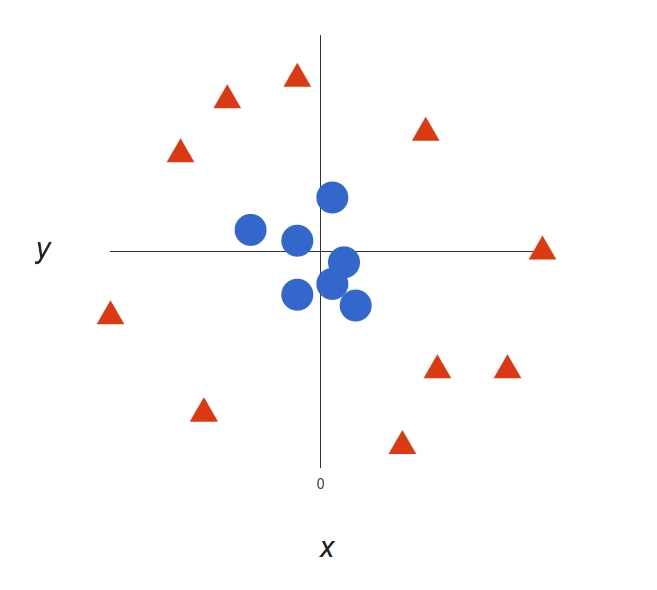
\includegraphics[width=.5\textwidth]{non-linear}
  \vspace*{3mm}
  \caption{Example of non-linearly separable data \parencite{svm-img}}
  \label{fig:non-linear}
\end{figure}
With computed histogram's for each image, a Support Vector Machine is used to train the classifier. The SVM algorithm attempts to find a hyperplane that separate classes with the highest possible margin \parencite{svm}. In the two dimensional Cartesian space a hyperplane would be a line however, since these hyperplanes are vectors this algorithm can be done at higher dimensions. However a Linear SVM would not be very helpful for this project since it attempts to classify five categories instead of two. This can be circumvented by adding more dimensions. For example, Figure \ref{fig:non-linear} shows a 2D example of non-linearly separable data. In this case, a 2D line cannot accurately separate these two categories. By using the equation for a circle $z=x^2+y^2$, a third $z$ dimension can be added. Mapped on a 2D $xz$ Cartesian plane, a clear linear hyperplane can be seen. See Figure \ref{fig:x-z-hyper}.
\begin{figure}[!h]
  \centering
  \captionsetup{justification=centering}
  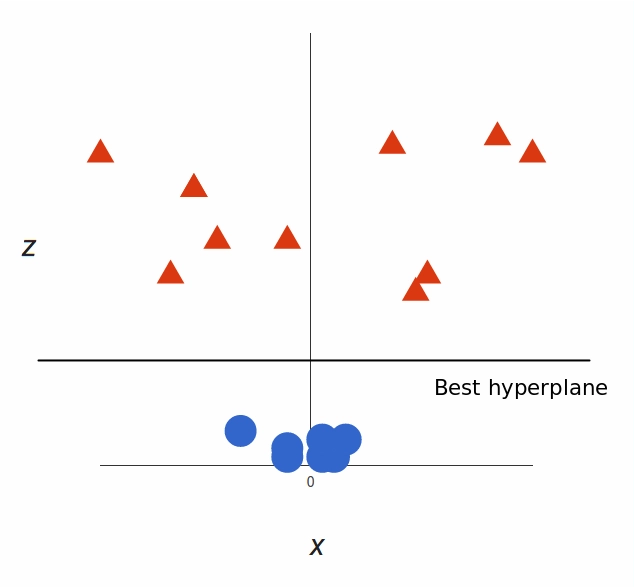
\includegraphics[width=.5\textwidth]{x-z-hyper}
  \vspace*{3mm}
  \caption{Example of linearly separable data in a higher dimension \parencite{svm-img}}
  \label{fig:x-z-hyper}
\end{figure}
In Figure \ref{fig:x-y-hyper}, this hyperplane and the data is mapped back into two dimensions, and circular decision boundary is generated.
\begin{figure}[!h]
  \centering
  \captionsetup{justification=centering, margin=2cm}
  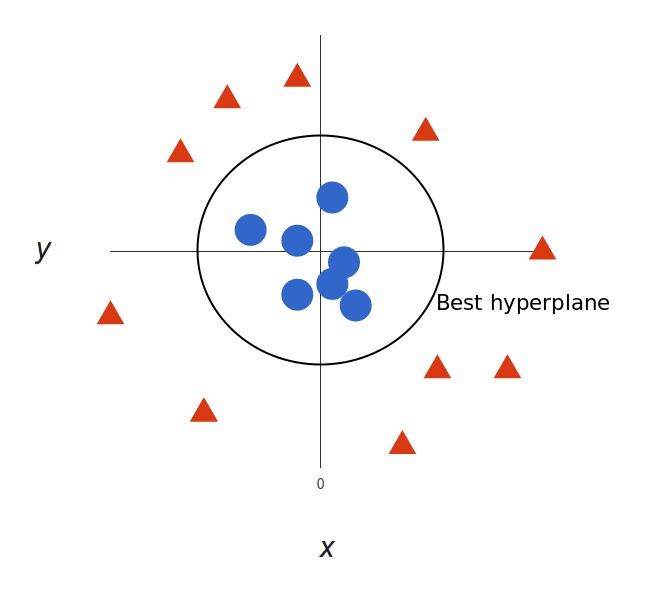
\includegraphics[width=.5\textwidth]{x-y-hyper}
  \vspace*{3mm}
  \caption{Example of using a kernel trick to linearly separate non-linearly separable data \parencite{svm-img}}
  \label{fig:x-y-hyper}
\end{figure}
\paragraph{Radial Based Function}
Mapping to higher dimensions to calculate vectors in a lower dimension for every support vector in the dataset can be very computationally expensive. A cheaper solution can be used called a Kernel Trick. The SVM algorithm doesn't need all of the entire dataset like a K-Nearest Neighborhood algorithm would, it just needs the support vectors during training. This means that only the dot products between the vectors. For example, in the previous example, the equations for a circle $z=x^2+y^2$ was used to add the third $z$ dimension to the problem. Rather than computing and storing new vectors every time another dimension is added, the dot product between these vectors can be calculated. The dot product of points $a$ and $b$ in this new $xyz$ dimension would be: $a \cdot b = xa \cdot xb + ya \cdot yb + za \cdot zb$. Simplifying the $z$ terms to lower $xy$ terms, the resulting computation is: $a \cdot b = xa \cdot xb + ya \cdot yb + (xa^2+ya^2) \cdot (xb^2+yb^2)$.
\subsection{Project Design}
The training pipeline is as follows: Images are first converted to gray scale. Keypoints are computed with a Oriented FAST algorithm and used to compute features using a Rotational BRIEF algorithm. Those feature vectors are clustered using a K-Means algorithm to develop a 64 word BoVW dictionary. This dictionary is then saved and is used to train with a SVM against the five category labels. Once the SVM regression is computed, it is saved for testing.\par
The testing pipeline is very similar to the training pipeline: Images are converted to gray scale. Keypoints are computed with oFAST and transformed to feature vectors with rBRIEF. Those features are clustered and vectorized with the K-Means model saved during training. Those vectors are then used to make a prediction on the saved SVM model.
\section{Results}
A few different training experiments were done to compare the efficiency and effectiveness of various parameters of the classifier. The most notable findings of these experiments was the comparison of the ORB algorithm vs the SIFT algorithm during the feature extraction step of the classifier. The control parameters of the two experiments were that: (1) All images in the dataset were used aside from the last 100 of each category reserved for testing (this is approximately a 83\%/17\% split). (2) All images were converted to gray scale using OpenCV's \verb|cvtColor| function with the \verb|COLOR_BGR2GRAY| option. (3) The features were clustered with the same K-Means clustering parameters were the number of clusters $n$ was 64. (4) The same parameters for the SVM and RBF were used in each experiment. (5) The K-Means and SVM models of each experiment was saved to disk using Python's standard library \verb|pickle| module. (6) All experiments were conducting on the same hardware: a Lenovo ThinkPad X1 Carbon with an Intel 8th Gen i7-8650U with 4 cores @ 4.2 GHz and 16 GB of RAM. The classifier was run with Python version 3.10.6 built on GCC version 11.3.0.\par
The first experiment used the SIFT algorithm to calculate keypoints and descriptors using OpenCV's built-in \verb|SIFT.detectAndCompute()| method. This detects keypoints and descriptors in one method call. Just the testing process of computing SIFT features for five-hundred images took just over four minutes. Computing the SIFT feature descriptors took nearly three times longer than training the SVM. Even after this terribly slow run time, it only had a classification rate of approximately 88\%.\par
The second experiment used the ORB algorithm to calculate keypoints and descriptors using OpenCV's built int \verb|ORB.detectAndCompute()| method. When testing on the five-hundred test images, computation took less than one minute during three separate training and testing runs. Accuracy of classification peaked at around 95\% with motorcycles being the category with the most misclassification. Of the one-hundred motorcycle testing images, nine of them were classified incorrectly. Six of those six were classified as cars with the last three being incorrectly classified as a airplanes. Cars preformed the best with an accuracy rate of 99\%, misclassifying only one image as a motorcycle.\par
The error rate of the motorcycle category is likely due to the fact that the car dataset was much larger and more detailed than the motorcycle dataset. More images plus more noise would lead to the classifier detecting more diverse features from the cars dataset. This means that the classifier is statistically more likely to be able to find more features it thinks are cars simply by the greater number of feature options it has seen. The same hypothesis can be used to explain the high classification rate of cars: by probability the classifier is more likely to classify an image as part of the car category.
\section{Conclusion}
Patented and slow feature extraction algorithms are not necessary for efficient computer vision projects. Neither is state-of-the-art graphics processing hardware. With open-source alternative ORB algorithm utilizing the oriented FAST and rotated BRIEF algorithms, feature extraction does not have to require high quality datasets nor multi-threaded hardware. This high-end hardware is also not needed to machine learning classification projects. With just a little bit of linear algebra kernel trickery, Support Vector Machines can be used to utilize their computational speed to classify more than just two categories. While SURF, SIFT, and Artificial Neural Networks may be the future of computer vision, low-cost efficient feature extraction and fast vector regression still represent a plethora of computer vision applications achievable by any student of computer science.
\printbibliography
\end{document}
